\section{Results}

When sampling the system, the correct $\Delta t$ must be selected which depends on the highest frequency which occurs in a time-reactive function in the whole system. For example in the SIR model we want infected agents to make on average contact with $\beta = 5$ other agents per time-unit, which means with a frequency of $\frac{1}{5}$. This functionality is built on Yampas function \textit{occasionally} which behaviour we investigated under differing $\Delta t$ with the above frequency. In this investigation we simply sampled occasionally with different $\Delta t$ for a duration of $t = 1,000$ and the event-frequency of $\frac{1}{5}$. The result can be seen in Figure \ref{fig:sampling_occasionally_5evts} and is quite striking. The plot clearly shows that occasionally needs a quite high sampling frequency even for a comparatively low event-frequency, which becomes of course worse for higher event-frequencies.

The other time-reactive function which occurs in the SIR model is the timed transition from infected to recovered which occurs on average with an exponential random-distribution after $\delta = 15$. This functionality is built on a custom implementation of Yampas \textit{after} which creates an event after a time-out of the passed in time-duration drawn from an exponential random-distribution. Clearly this function has different semantics as although it also continuously emit events over time - \textit{NoEvent} before the time was hit, and \textit{Event b} after the time hit - the relevant point is that it switches to Event at some discrete point in time. This is implemented as simply adding up the $\Delta t$ until the accumulator is greater of equal than the previously drawn exponential time-out. We also investigated the behaviour of this function under varying $\Delta t$ using a time-out of $\delta = 15$. Our approach was to sample the \textit{afterExp} until an event occurs and then see when it has occurred. We run this with 10,000 replications with different random-number seeds and average the resulting times. The results can be seen in Figure \ref{fig:sampling_afterExp_5time}. The result is striking in another way: this function seems to be pretty invariant to the time-deltas, for obvious reasons: we are basically just interested in the "after"-condition of the whole semantics whereas in occasionally we are interested in the "repeatedly"-conditions. If we under-sample the \textit{afterExp} then we can be off by one $\Delta t$. If we under-sample \textit{occasionally} we keep loosing events - the less difference between $\Delta t$ and event-frequency, the more events we lose. Of course \textit{afterExp} can also be used for very short time-outs e.g. $\frac{1}{5}$. We have investigated the behaviour of this function for various $\Delta t$ as well as seen in Figure \ref{fig:sampling_afterExp_02time}. Here the result is much more striking and shows that \textit{afterExp} is vulnerable to small time-outs as well as \textit{occasionally}.  
To show that \textit{occasionally} is not vulnerable to very low frequencies of e.g. one event every 5 time-steps we plotted the behaviour of this under varying time-steps in Figure \ref{fig:sampling_occasionally_02evts}. The result shows that for low frequencies occasionally works fine with larger $\Delta t$.

\begin{figure}
\begin{center}
	\begin{tabular}{c c}
	\begin{subfigure}[b]{0.5\textwidth}
			\centering
			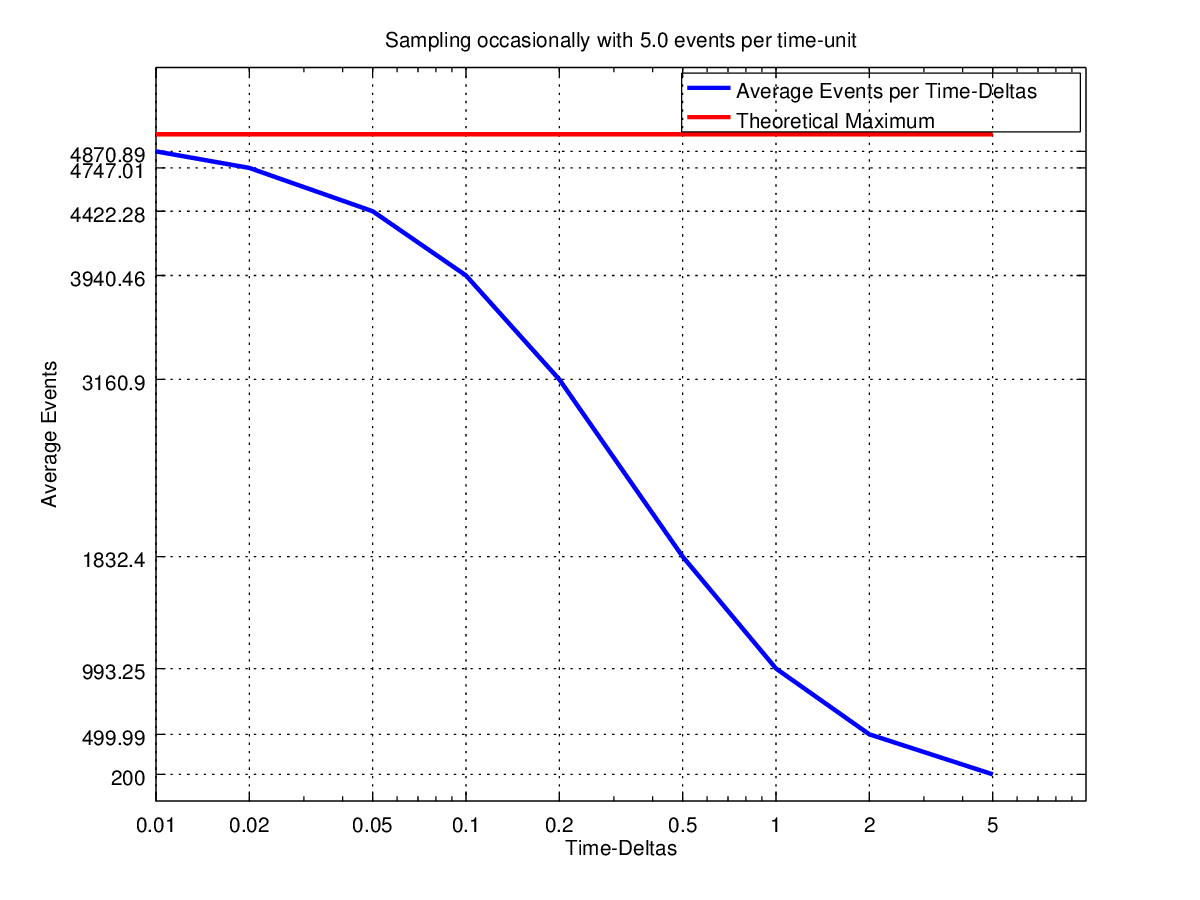
\includegraphics[width=.6\textwidth, angle=0]{./../shared/fig/sampling/samplingTest_occasionally_5evts.png}
			\caption{Sampling \textit{occasional} with a frequency of $\frac{1}{5}$ (average of 5 events per time-unit). The theoretical average is 5000 events within this time-frame.}
			\label{fig:sampling_occasionally_5evts}
		\end{subfigure}
		& 
		\begin{subfigure}[b]{0.5\textwidth}
			\centering
			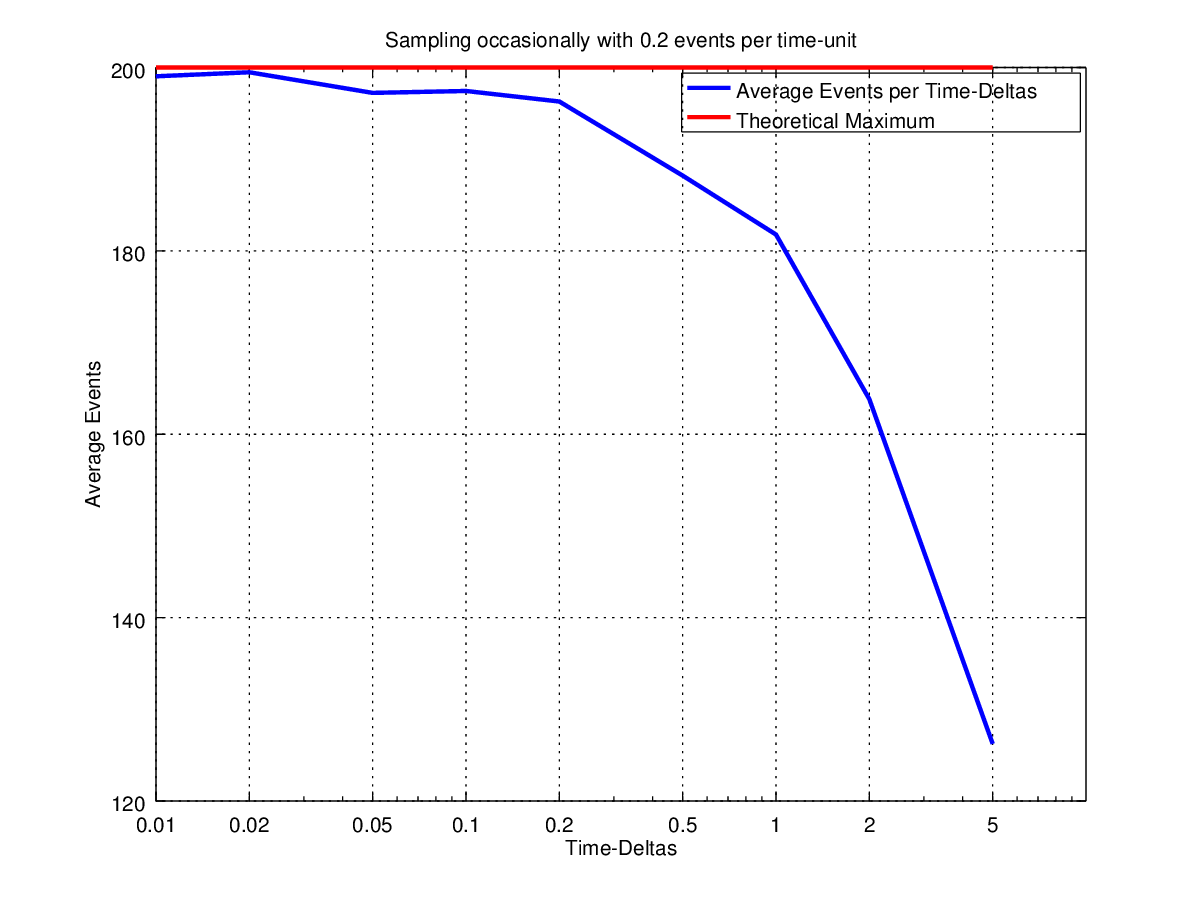
\includegraphics[width=.6\textwidth, angle=0]{./../shared/fig/sampling/samplingTest_occasionally_02evts.png}
			\caption{Sampling \textit{occasional} with a frequency of 5 (average of 0.2 events per time-unit). The theoretical average is 200 events within this time-frame.}
			\label{fig:sampling_occasionally_02evts}
		\end{subfigure}
		
		\\
		
		\begin{subfigure}[b]{0.5\textwidth}
			\centering
			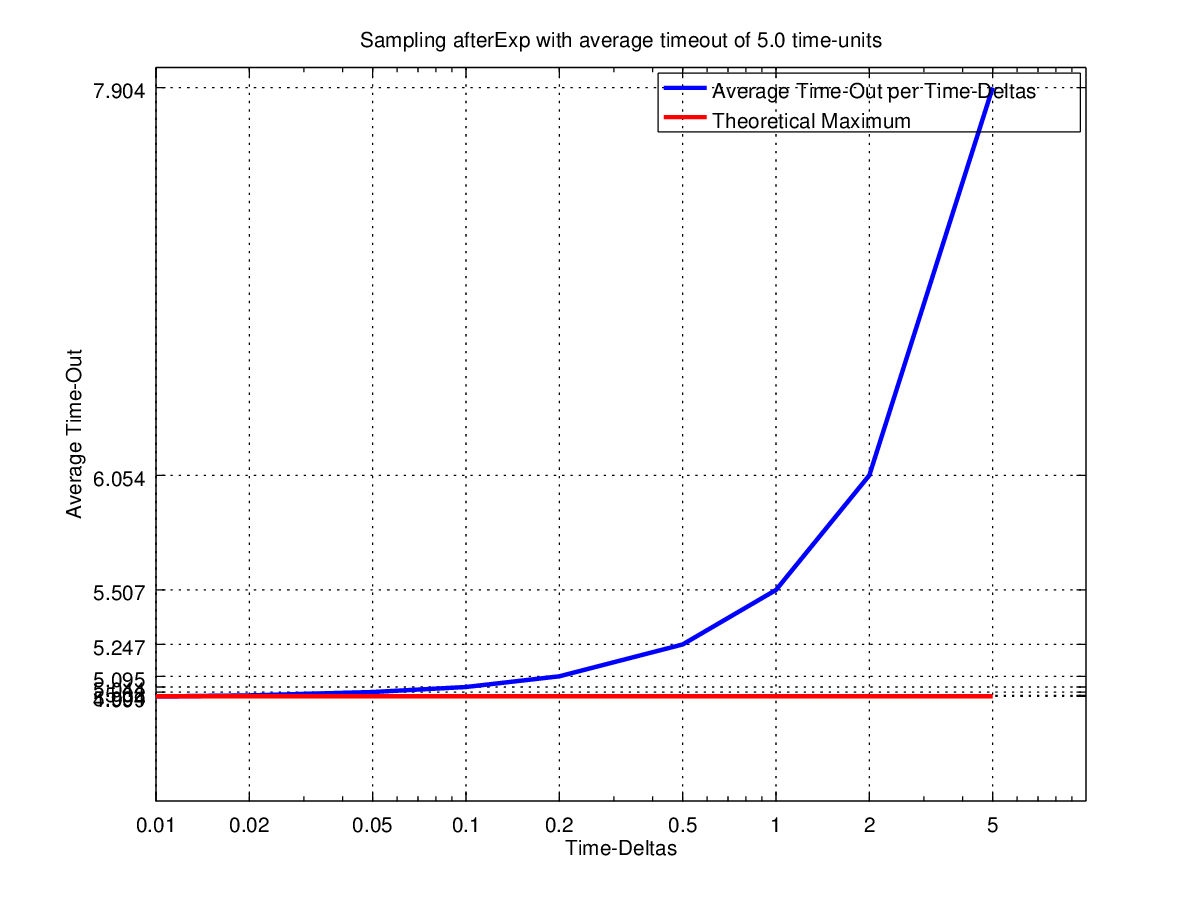
\includegraphics[width=.6\textwidth, angle=0]{./../shared/fig/sampling/samplingTest_afterExp_5time.png}
			\caption{Sampling \textit{afterExp} with an average time-out of 5.}
			\label{fig:sampling_afterExp_5time}
		\end{subfigure}
		& 
		\begin{subfigure}[b]{0.5\textwidth}
			\centering
			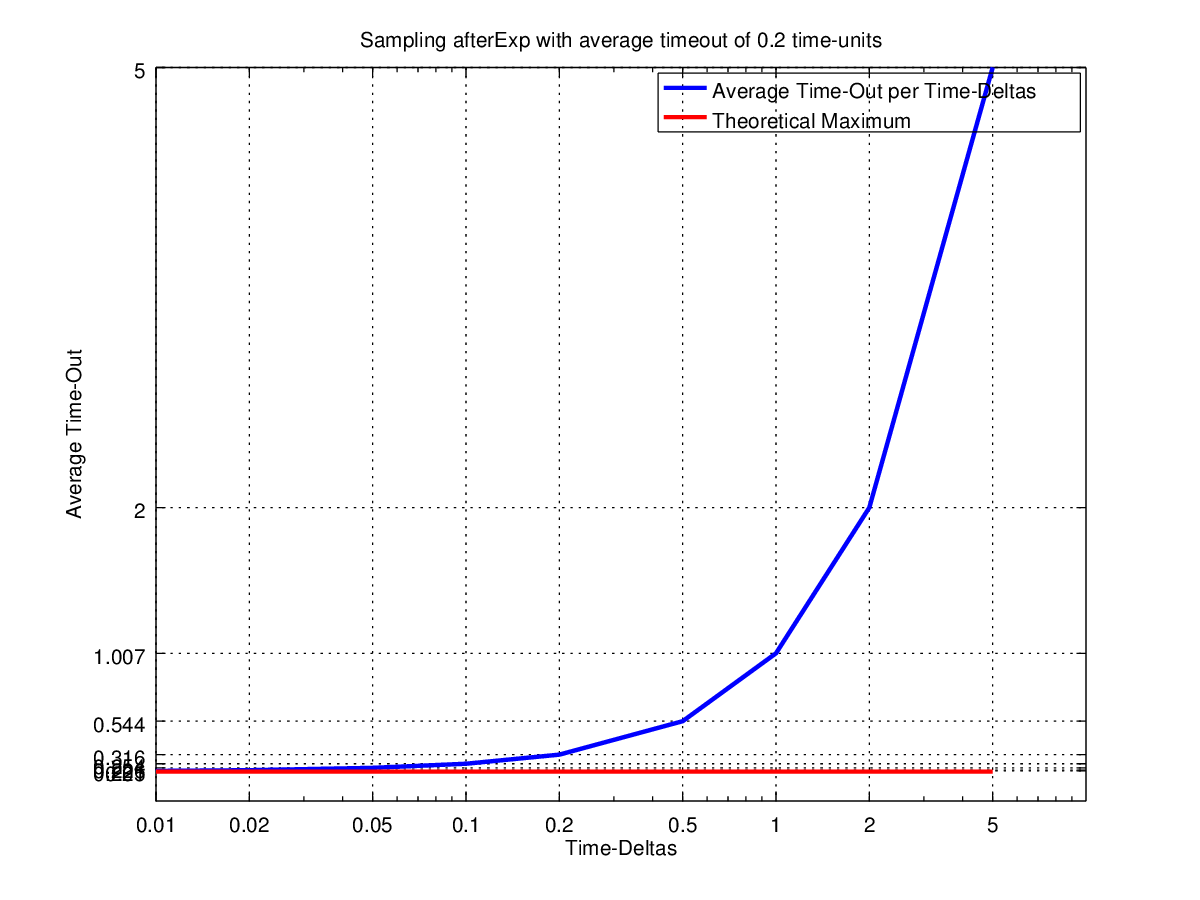
\includegraphics[width=.6\textwidth, angle=0]{./../shared/fig/sampling/samplingTest_afterExp_02time.png}
			\caption{Sampling \textit{afterExp} with an average time-out of 0.2.}
			\label{fig:sampling_afterExp_02time}
		\end{subfigure}
	\end{tabular}
	
	\caption{Sampling the \textit{afterExp} and \textit{occasional} functions to visualise the influence of sampling frequencies on the occurrence of the respective events. $\Delta t$ are [ 5, 2, 1, $\frac{1}{2}$, $\frac{1}{5}$, $\frac{1}{10}$, $\frac{1}{20}$, $\frac{1}{50}$, $\frac{1}{100}$ ]. The experiments for \textit{afterExp} used 10,000 replications. The experiments for \textit{occasional} ran for $t= 1,000$ with 100 replications.} 
	\label{fig:sampling_tests}
\end{center}
\end{figure}

\subsection{Increasing the frequency}
Using these observation we run simulations with varying $\Delta t$ with $\Delta = 0.5$, $\Delta = 0.2$ and $\Delta = 0.1$ with the results visible in Figures \ref{fig:sir_abs_approximating_05dt}, \ref{fig:sir_abs_approximating_02dt} and \ref{fig:sir_abs_approximating_01dt} but still when decreasing $\Delta t$ we don't approach the SD dynamics. As previously mentioned the agent-based approach is a discrete one which means that with increasing number of agents, the discrete dynamics approximate the continuous dynamics of the SD simulation. We run further simulations with $\Delta = 0.1$ but with varying agent numbers to see the influence with the results seen in Figure \ref{fig:sir_abs_approximating}.

\begin{figure}
\begin{center}
	\begin{tabular}{c c}
		\begin{subfigure}[b]{0.3\textwidth}
			\centering
			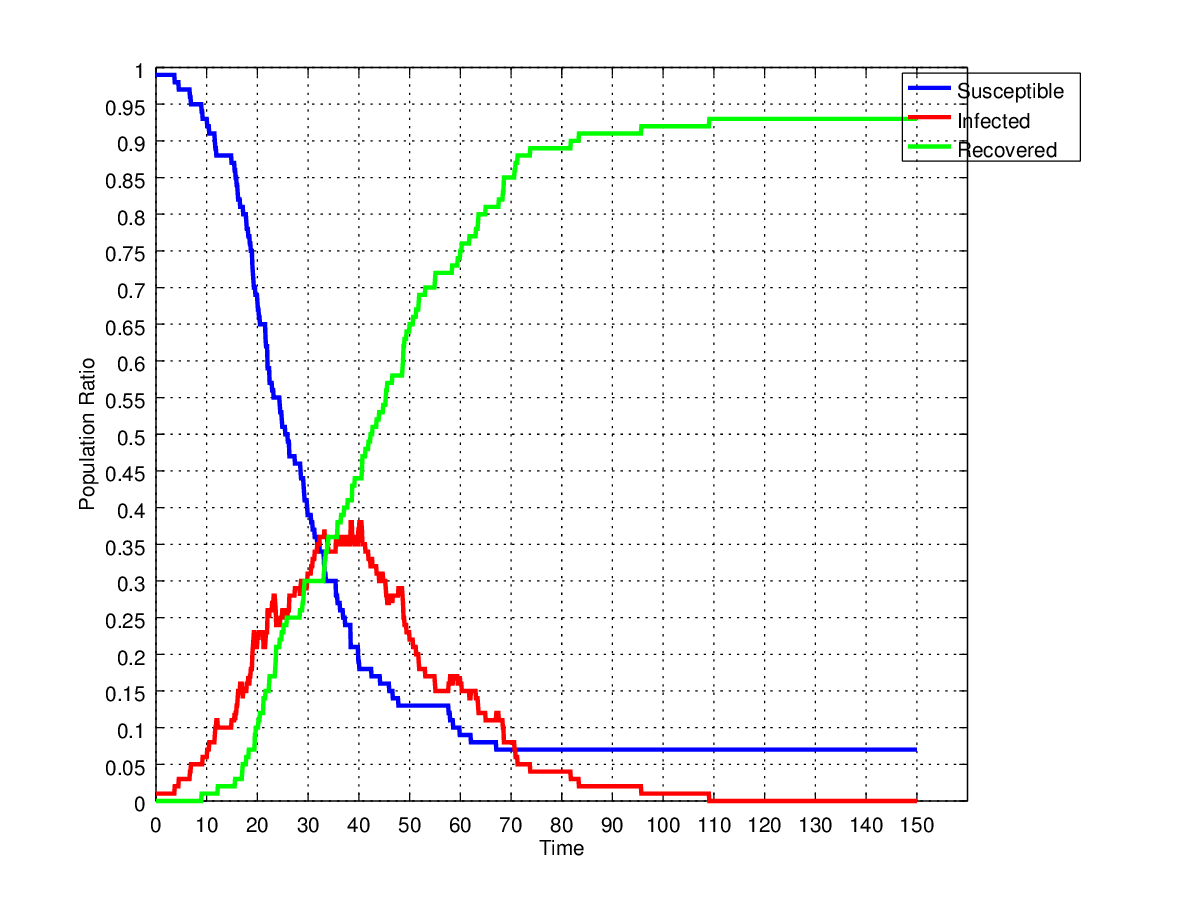
\includegraphics[width=1\textwidth, angle=0]{./../shared/fig/frabs/SIR_100agents_150t_01dt_NOSS_parallel.png}
			\caption{100 Agents}
			\label{fig:sir_abs_approximating_100}
		\end{subfigure}
    	&
		\begin{subfigure}[b]{0.3\textwidth}
			\centering
			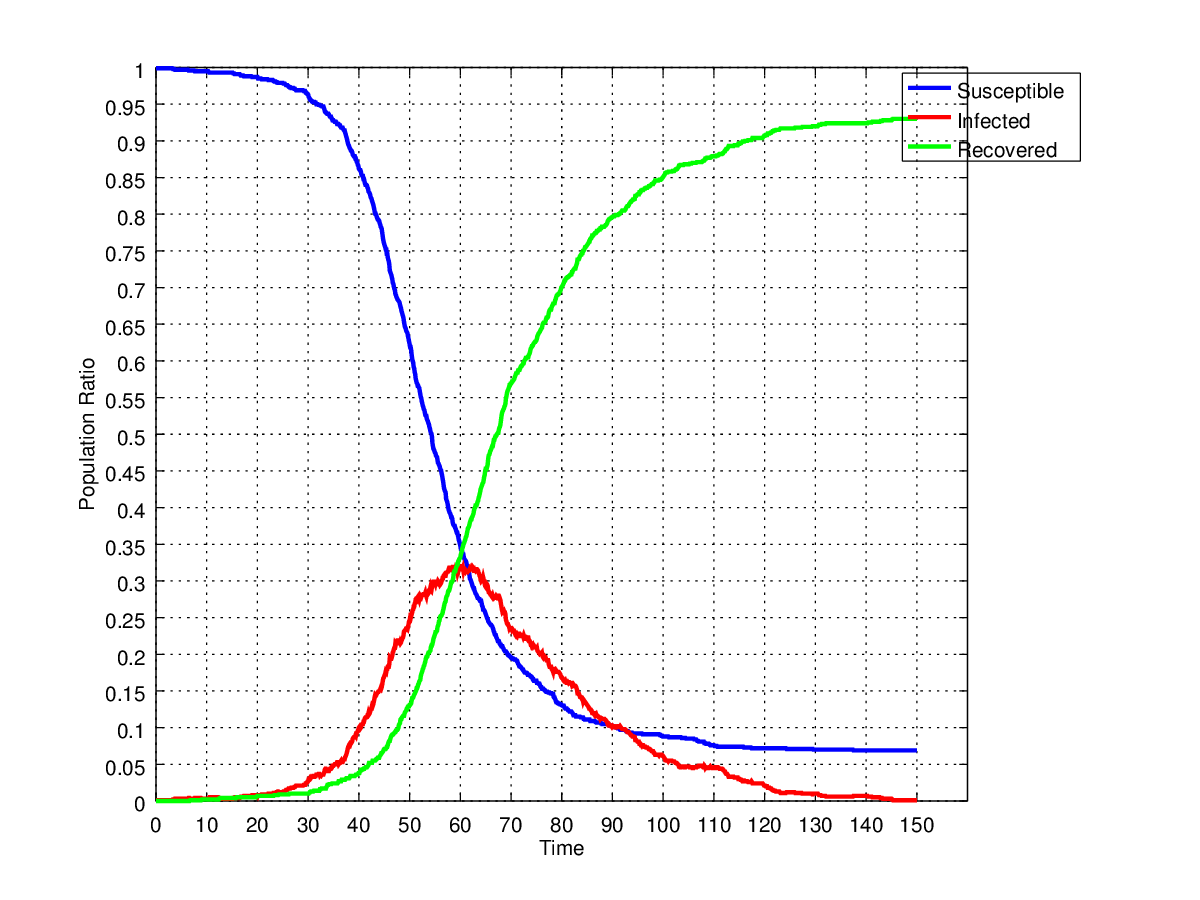
\includegraphics[width=1\textwidth, angle=0]{./../shared/fig/frabs/SIR_1000agents_150t_01dt_NOSS_parallel.png}
			\caption{1,000 Agents}
			\label{fig:sir_abs_approximating_1000}
		\end{subfigure}
    	
    	\\
    	
		\begin{subfigure}[b]{0.3\textwidth}
			\centering
			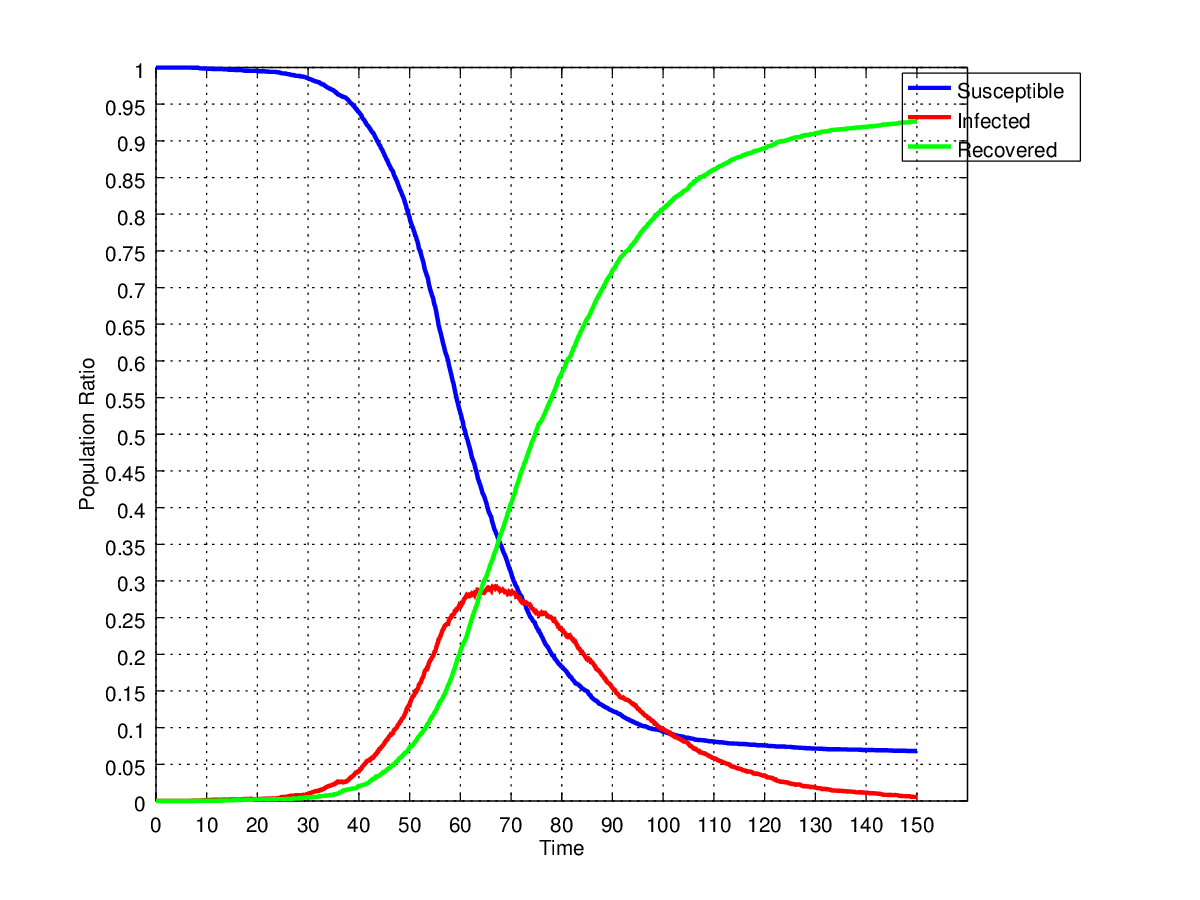
\includegraphics[width=1\textwidth, angle=0]{./../shared/fig/frabs/SIR_5000agents_150t_01dt_NOSS_parallel.png}
			\caption{5,000 Agents}
			\label{fig:sir_abs_approximating_5000}
		\end{subfigure}
		& 
		\begin{subfigure}[b]{0.3\textwidth}
			\centering
			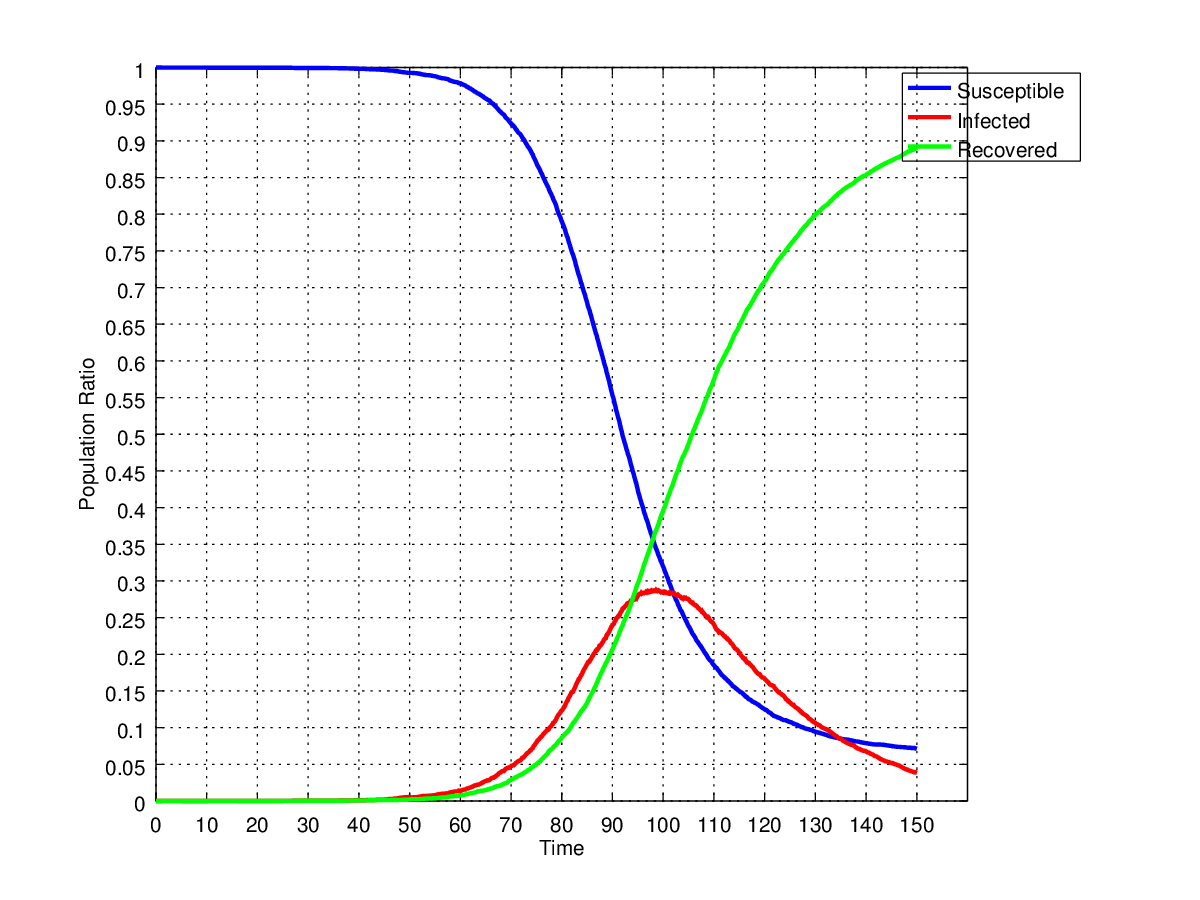
\includegraphics[width=1\textwidth, angle=0]{./../shared/fig/frabs/SIR_10000agents_150t_01dt_NOSS_parallel.png}
			\caption{10,000 Agents}
			\label{fig:sir_abs_approximating_10000}
		\end{subfigure}
	\end{tabular}
	
	\caption{Varying agent numbers with same model-parameters except population size. All simulations run for 150 time-steps with $\Delta t = 0.1$}
	\label{fig:sir_abs_approximating}
\end{center}
\end{figure}

Although increasing the number of agents improves our approximation, still the dynamics of 10,000 Agents are still nowhere close to the SD dynamics. This is because as opposed to SD, which is deterministic, the agent-based approach is inherently a stochastic one as we continuously draw from random-distributions which drive our state-transitions. What we see in Figure \ref{fig:sir_abs_approximating} is then just a single run where the dynamics would result in slightly different shapes when run with a different random-number generator seed. The agent-based approach thus generates a distribution of dynamics over which ones needs to average to arrive at the correct solution. 